\subsection{Упражнение 1}

Показать на графике время работы analyze1 и analyze2 в логарифмическом масштабе. Сравнить с scipy.fftpack.dct.

\begin{lstlisting}[language=Python]
def analyze1(ys, fs, ts):
    args = np.outer(ts, fs)
    M = np.cos(PI2 * args)
    amps = np.linalg.solve(M, ys)
    return amps
def analyze2(ys, fs, ts):
    args = np.outer(ts, fs)
    M = np.cos(PI2 * args)
    amps = M.dot(ys) / 2
    return amps
\end{lstlisting}

Зазадим размер массива степенями двойки.

\begin{lstlisting}[language=Python]
ns = 2 ** np.arange(5,10)
\end{lstlisting}

\begin{lstlisting}[language=Python]
best_analyze1 = []
for n in ns:
    ts = (0.5 + np.arange(n)) / n
    freqs = (0.5 + np.arange(n)) / 2
    ys = wave.ys[:n]
    best =  %timeit -r1 -o analyze1(ys,freqs,ts)
    best_analyze1.append(best.best)
best_analyze2 = []
for n in ns:
    ts = (0.5 + np.arange(n)) / n
    freqs = (0.5 + np.arange(n)) / 2
    ys = wave.ys[:n]
    best =  %timeit -r1 -o analyze2(ys,freqs,ts)
    best_analyze2.append(best.best)
best_dct = []
for n in ns:
    ys = wave.ys[:n]
    best =  %timeit -r1 -o scipy.fftpack.dct(ys, type=3)
    best_dct.append(best.best)
plt.plot(ns, best_analyze1, label='analyze1')
plt.plot(ns, best_analyze2, label='analyze2')
plt.plot(ns, best_dct, label='fftpack.dct')
loglog = dict(xscale='log', yscale='log')
decorate(xlabel='Wave length (N)', ylabel='Time (s)', **loglog)
\end{lstlisting}

\begin{figure}[H]
	\begin{center}
		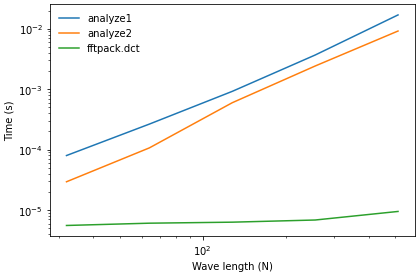
\includegraphics[scale=1]{fig/lab06/lab6_1.png}
		\caption{Время работы различных методов ДКП}
	\end{center}
\end{figure}

Не смотря на теоритическое время исполнения, время analyze1 получилсось пропорциональным  n2 .

\subsection{Упражнение 2}

Реализовать алгоритм сжатия для музыки или речи.

Выберем звук для сжатия:
\begin{lstlisting}[language=Python]
if not os.path.exists('1647_piano.wav'):
    !wget https://github.com/pimenov01/telecom/raw/main/files/1647_piano.wav
    wave = read_wave('1647_piano.wav')
\end{lstlisting}

Для начала возьмём небольшой сегмент:

\begin{lstlisting}[language=Python]
segment = wave.segment(start = 1.7,duration = 1.0)
segment.normalize()
segment.make_audio()
\end{lstlisting}

Используем DCT вместо DFT.

\begin{lstlisting}[language=Python]
dct = segment.make_dct()
dct.plot(high = 5000)
\end{lstlisting}
\begin{figure}[H]
	\begin{center}
		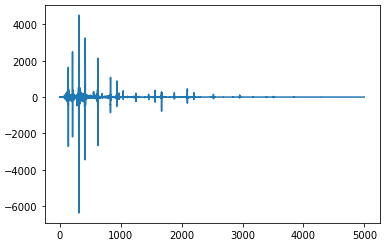
\includegraphics[scale=1]{fig/lab06/lab6_2.png}
		\caption{Спектр сигнала полученный при помощи ДКП}
	\end{center}
\end{figure}

\begin{lstlisting}[language=Python]
def filtering(dct,limit = 0):
  for i, amp in enumerate(dct.amps):
    if np.abs(amp) < limit:
      dct.hs[i] = 0
\end{lstlisting}

\begin{lstlisting}[language=Python]
filtering(dct,1000)
dct.plot(high = 5000)
\end{lstlisting}
\begin{figure}[H]
	\begin{center}
		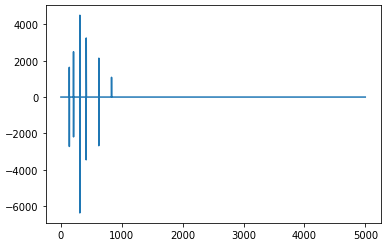
\includegraphics[scale=1]{fig/lab06/lab6_3.png}
		\caption{ДКП после фильтрации}
	\end{center}
\end{figure}

Теперь подберём значение, чтобы результат звучал как исходник. Для эффективного хранения данных можно использовать разряженные массивы.

\subsection{Управжнение 3}

В блокноте phase.ipynb взять другой сегмент звука и повторить эксперименты.

\begin{lstlisting}[language=Python]
signal = SawtoothSignal(freq=500, offset=0)
wave = signal.make_wave(duration=0.5, framerate=40000)
wave.segment(start=0.005,duration=0.01).plot()
decorate(xlabel='Time (s)')
\end{lstlisting}
\begin{figure}[H]
	\begin{center}
		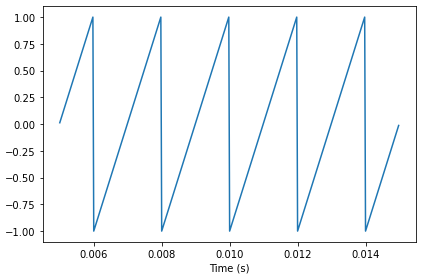
\includegraphics[scale=1]{fig/lab06/lab6_4.png}
		\caption{Выбранный сегмент}
	\end{center}
\end{figure}

\begin{lstlisting}[language=Python]
spectrum = wave.make_spectrum()
spectrum.plot()
decorate(xlabel='Frequency (Hz)',
         ylabel='Amplitude')
\end{lstlisting}
\begin{figure}[H]
	\begin{center}
		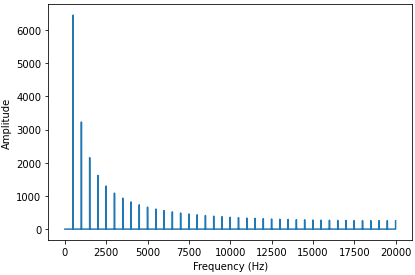
\includegraphics[scale=1]{fig/lab06/lab6_5.png}
		\caption{Спектр сегемента}
	\end{center}
\end{figure}

\begin{lstlisting}[language=Python]
def plot_angle(spectrum, thresh=1):
    angles = spectrum.angles
    angles[spectrum.amps < thresh] = np.nan
    plt.plot(spectrum.fs, angles, 'x')
    decorate(xlabel='Frequency (Hz)', 
             ylabel='Phase (radian)')
             
def plot_three(spectrum, thresh=1):
    """Plot amplitude, phase, and waveform.
    
    spectrum: Spectrum object
    thresh: threshold passed to plot_angle
    """
    plt.figure(figsize=(10, 4))
    plt.subplot(1,3,1)
    spectrum.plot()
    plt.subplot(1,3,2)
    plot_angle(spectrum, thresh=thresh)
    plt.subplot(1,3,3)
    wave = spectrum.make_wave()
    wave.unbias()
    wave.normalize()
    wave.segment(duration=0.01).plot()
    display(wave.make_audio())

def zero_angle(spectrum):
    res = spectrum.copy()
    res.hs = res.amps
    return res
    
def rotate_angle(spectrum, offset):
    res = spectrum.copy()
    res.hs *= np.exp(1j * offset)
    return res

def random_angle(spectrum):
    res = spectrum.copy()
    angles = np.random.uniform(0, PI2, len(spectrum))
    res.hs *= np.exp(1j * angles)
    return res
\end{lstlisting}

\begin{lstlisting}[language=Python]
plot_three(spectrum)
\end{lstlisting}
\begin{figure}[H]
	\begin{center}
		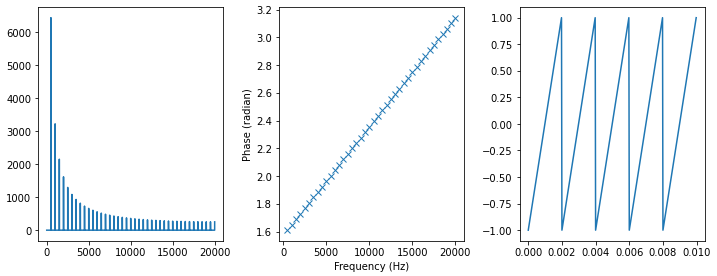
\includegraphics[scale=0.66]{fig/lab06/lab6_6.png}
		\caption{Получившиеся графики}
	\end{center}
\end{figure}

\begin{lstlisting}[language=Python]
spectrum2 = zero_angle(spectrum)
plot_three(spectrum2)
\end{lstlisting}
\begin{figure}[H]
	\begin{center}
		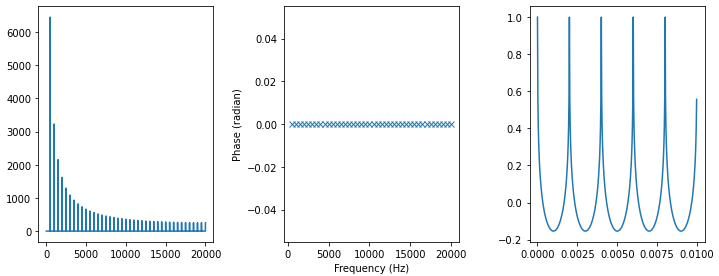
\includegraphics[scale=0.66]{fig/lab06/lab6_7.png}
		\caption{Получившиеся графики}
	\end{center}
\end{figure}


\begin{lstlisting}[language=Python]
spectrum3 = rotate_angle(spectrum, 1)
plot_three(spectrum3)
\end{lstlisting}
\begin{figure}[H]
	\begin{center}
		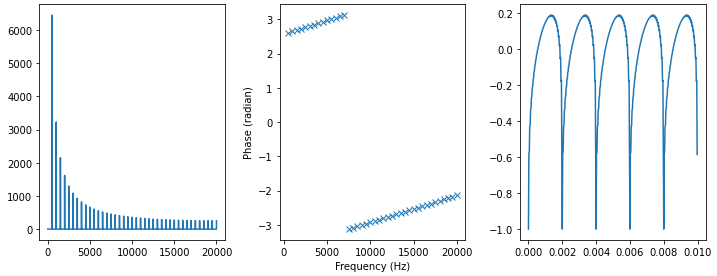
\includegraphics[scale=0.66]{fig/lab06/lab6_8.png}
		\caption{Получившиеся графики}
	\end{center}
\end{figure}


\begin{lstlisting}[language=Python]
spectrum4 = random_angle(spectrum)
plot_three(spectrum4)
\end{lstlisting}
\begin{figure}[H]
	\begin{center}
		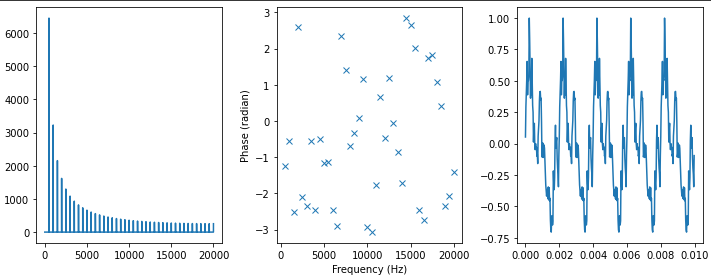
\includegraphics[scale=0.66]{fig/lab06/lab6_9.png}
		\caption{Получившиеся графики}
	\end{center}
\end{figure}

Теперь возьмём другой звук и сделаем всё тоже самое:

\begin{lstlisting}[language=Python]
if not os.path.exists('120994__thirsk__120-oboe.wav'):
    !wget https://github.com/AllenDowney/ThinkDSP/raw/master/code/120994__thirsk__120-oboe.wav
wave = read_wave('120994__thirsk__120-oboe.wav')
segment = wave.segment(start=0.1, duration=0.5)
spectrum = segment.make_spectrum()
\end{lstlisting}

\begin{lstlisting}[language=Python]
plot_three(spectrum)
\end{lstlisting}
\begin{figure}[H]
	\begin{center}
		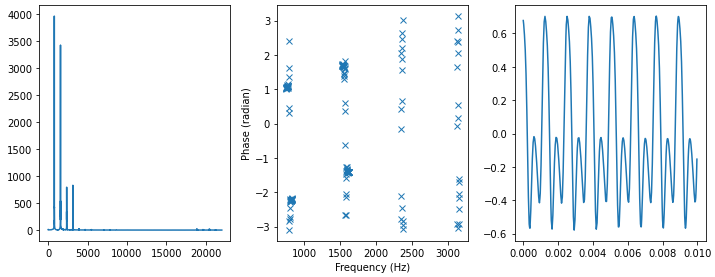
\includegraphics[scale=0.66]{fig/lab06/lab6_10.png}
		\caption{Получившиеся графики}
	\end{center}
\end{figure}

\begin{lstlisting}[language=Python]
spectrum2 = zero_angle(spectrum)
plot_three(spectrum2)
\end{lstlisting}
\begin{figure}[H]
	\begin{center}
		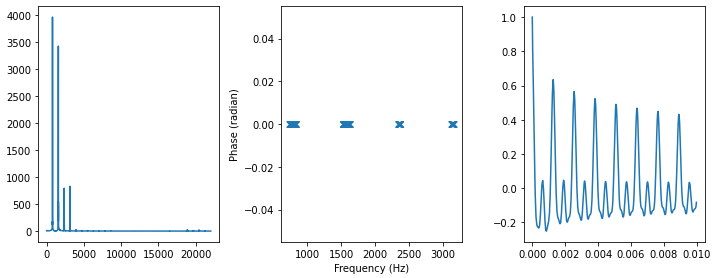
\includegraphics[scale=0.66]{fig/lab06/lab6_11.png}
		\caption{Получившиеся графики}
	\end{center}
\end{figure}


\begin{lstlisting}[language=Python]
spectrum3 = rotate_angle(spectrum, 1)
plot_three(spectrum3)
\end{lstlisting}
\begin{figure}[H]
	\begin{center}
		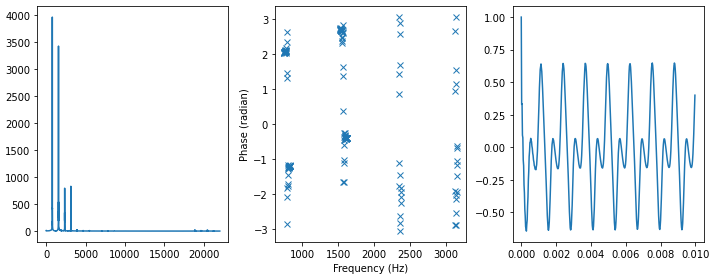
\includegraphics[scale=0.66]{fig/lab06/lab6_12.png}
		\caption{Получившиеся графики}
	\end{center}
\end{figure}


\begin{lstlisting}[language=Python]
spectrum4 = random_angle(spectrum)
plot_three(spectrum4)
\end{lstlisting}
\begin{figure}[H]
	\begin{center}
		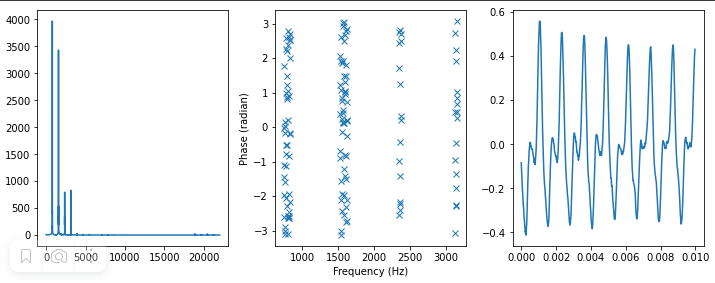
\includegraphics[scale=0.66]{fig/lab06/lab6_13.png}
		\caption{Получившиеся графики}
	\end{center}
\end{figure}

Звук при прослушивании остался таким же, хотя мы изменили сигнал достаточно сильно. Если гармоническая структура звука неизменна - то для звуков с простой структурой мы не услышим изменений в фазовой структуре.

\subsection{Вывод}

ДКП применяется в MP3 и соответвующих форматах сжатия музыки, в JPEG, MPEG и так далее. ДКП похоже на ДПФ, использованное в спектральном анализе. Также при помощи ДКП были исследованы свойства звуков с разной структурой.